\section{Physical view}
In de physical view wordt er gekeken naar hoe het systeem gedeployed moet worden en waar.
Om dit in beeld te brengen is er gebruikgemaakt van een deployment diagram \ref{fig:DeploymentDiagram}.
Er is gekozen om gebruik te maken van Docker \Parencite{Docker}.
Docker is een softwareoplossing waarmee software gedeployed kan worden op elke machine via een lichte en efficiënte manier \Parencite{Docker}.
Door gebruik te maken van docker kan het systeem gemakkelijk gedeployed worden op cloud hosting platformen en dynamisch schalen.

\whitespace
\begin{graphic}
    \captionsetup{type=figure}
    \caption{Deployment diagram van het afstudeerproduct}
    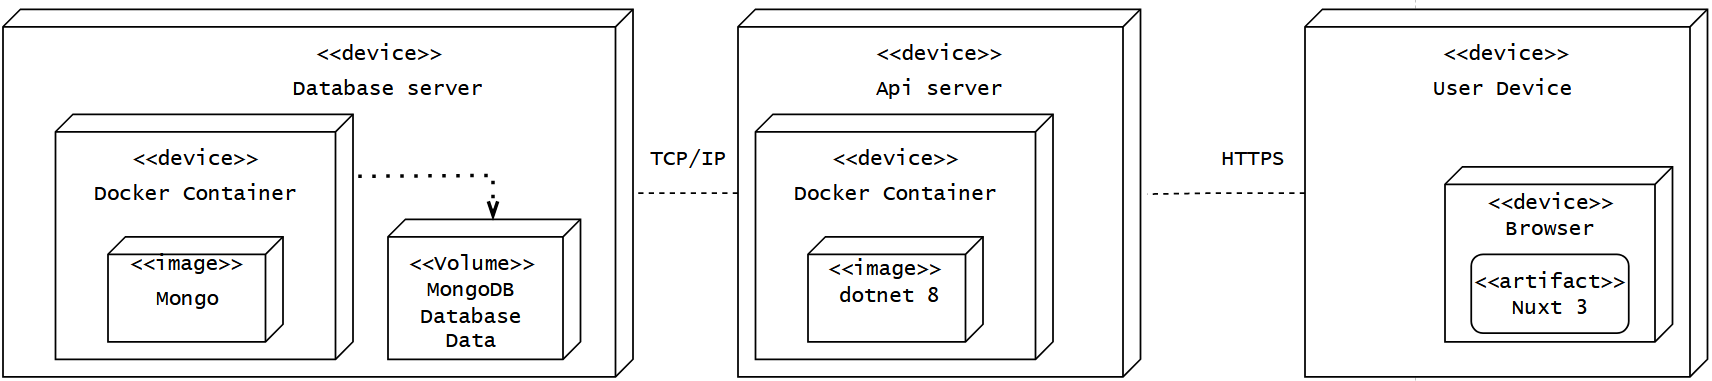
\includegraphics[scale=0.37]{DeploymentDiagram.png}
    \label{fig:DeploymentDiagram}
\end{graphic}
